\documentclass{article}
\usepackage{amsmath}
\usepackage{amssymb}
\usepackage{array}
\usepackage{caption}
\usepackage{enumitem}
\usepackage[margin=1.0in]{geometry}
\usepackage{graphicx}
\usepackage{mathtools}
\usepackage{multirow}
\usepackage{subcaption}
\usepackage{tabularx}
\usepackage{verbatim}
\usepackage{colortbl}
\usepackage[table]{xcolor}

\definecolor{myGray}{gray}{0.8}

\newcommand\rankeq{\mathrel{\overset{\makebox[0pt]{\mbox{\normalfont\tiny\sffamily rank}}}{=}}}

\setlist[itemize]{noitemsep}  % remove space between list items

\begin{document}

\author{Garrick Sherman}

\title{Document Expansion with External Collections for Information Retrieval}

\maketitle
\begin{abstract}
\end{abstract}

\section{Introduction}\label{section.intro}

When using language models (LMs) to perform document retrieval, we treat the query and document texts as observations from unseen (and unobservable) probabilistic processes. In the query likelihood (QL) retrieval model, we rank each document by the likelihood that its language model would ``generate'' the query text. However, if the query is a sample from an underlying stochastic process, it is generally too sparse to fully represent an informtion need.

Relevance modeling is an extremely influential pseudo-relevance feedback technique that helps to allievate the problem of vocabulary mismatch. Instead of assuming that queries are observations sampled from \textit{document} models, we assume that both queries and documents are observations sampled from a \textit{relevance} model (RM) \cite{Lavrenko2001}. We can use this idea to expand the query representation into an estimate of the relevance model as explained in Section \ref{section.expanding.model.rm} and rank documents by the similarity of their estimated language model to the estimated RM.

As a form of pseudo-relevance feedback, part of the relevance modeling process involves assuming that top-ranked documents are relevant to the query. Although this assumption is generally untrue, it is true of enough top-ranked documents that the estimated RM will be of good quality. That is, initially retrieved documents provide a good estimate of the underlying relevance model \textit{in their aggregate}; taken individually, documents are not assumed to accurately represent the underlying RM.

We suggest that, given that a top-ranked document is, like a query, considered a limited observation of terms from a relevance model, documents may be expanded to better reflect their underlying relevance model. In this paper, we propose a method of document expansion that closely mirrors the process of relevance modeling. This document expansion process serves many of the same roles as traditional relevance modeling without excluding the use of RMs; indeed, our document expansion process is complementary to query expansion.

\textbf{Talk about external collections and combining evidence.}

\section{Related Work}\label{section.related}

\subsection{Document Expansion in IR}\label{section.related.ir}

Prior work

Our idea is related to Wei and Croft's LDA-based document model, which smooths the document language model with latent Dirichlet allocation probabilities \cite{Wei2006}. Liu and Croft's \textit{CBDM} model performs a similar type of document expansion by interpolating the probability of a query term in a document cluster with its probability in the document \cite{Liu2004}.

Most similar to our approach is that of Efron, Organisciak and Fenlon \cite{Efron2012}.

\subsection{Incorporating External Collections}\label{section.external.collections}

\cite{Diaz2006} introduces the use of external collections to relevance modeling.

\section{Document Expansion Procedure}\label{section.expanding}

\subsection{Underlying Retrieval Model}\label{section.expanding.model}
Throughout this paper we rely on the language modeling retrieval framework \cite{Lafferty2001}, though this is not strictly necessary and imposes no particular mathematical constraints on our approach. More specifically, we employ the query likelihood (QL) and relevance modeling ranking methods. 

\subsubsection{Query Likelihood}\label{section.expanding.model.ql}

Given a query $Q$ and a document $D$, we rank documents on $P(Q | \theta_D)$, where $\theta_D$ is the language model (typically a multinomial over the vocabulary $V$) that generated the text of document $D$.  Assuming independence among terms and a uniform distribution over documents, each document is scored by

\begin{flalign}\label{equation.ql}
\log P(Q | D) = \prod_{w \in Q} P(w | Q) \cdot \log P(w | \theta_D) .
\end{flalign}

\noindent We follow standard procedures for estimating the probabilities in Eq. \ref{equation.ql}.  We simply use the maximum likelihood estimate of $\hat{P}(w | Q) = \frac{c(w, Q)}{|Q|}$ where $c(w, Q)$ is the frequency of word $w$ in $Q$.  For $P(w | \theta_D)$ we estimate a smoothed language model by assuming that document language models
in a given collection have a Dirichlet prior distribution:

\begin{flalign}\label{equation.ql-dirichlet}
\hat{P}(w | \theta_D) = \frac{c(w, D) + \mu \hat{P}(w | C)}{|D| + \mu} 
\end{flalign}

\noindent where $\hat{P}(w | C)$ is the maximum likelihood estimate of the probability of seeing word $w$ in a ``background" collection $C$ (typically $C$ is the corpus from which $D$ is drawn), and $\mu \geq 0$ is the smoothing hyper-parameter. 

\subsubsection{Relevance Modeling}\label{section.expanding.model.rm}

Relevance modeling is a form of pseudo-relevance feedback that uses top ranked documents to estimate a language model representing documents relevant to a query \cite{Lavrenko2001}. This language model, known as a relevance model, acts as a form of query expansion and is generally used with the KL divergence retrieval model \cite{Zhai2006} to score documents.

A relevance model takes the form of

\begin{flalign}\label{equation.rm1}
	P(w|R) = \sum_{D \in C} P(D) P(w|D) P(Q|D)
\end{flalign}

\noindent where $P(Q|D)$ is calculated as in Equation \ref{equation.ql} and essentially weights word $w$ in document $D$ by the query likelihood of the document. Though theoretically calculated over all words and documents, relevance models are more efficient and robust when calculated over only the top terms in only the top ranked documents. These parameters are referred to as $fbTerms$ and $fbDocs$ respectively in Table \ref{table.parameters}.

Because relevance models are prone to query drift, research has shown that linearly interpolating a relevance model with the original query model to improve performance:

\begin{flalign}\label{equation.rm3}
	P(w|Q') = (1-\alpha) P(w|R) + \alpha P(w|Q).
\end{flalign}

\noindent $\alpha$ is a mixing parameter controlling the influence of the original query. This form of relevance model is known as ``RM3'' and is the baseline used throughout this paper.

\subsection{Expanding with Document Pseudo-Queries}\label{section.expanding.queries}

To expand a document $D$, we begin by treating the text of $D$ as a pseudo-query which we pose against a collection of documents $C_E$.  To transform a document into a pseudo-query we apply two transformations.  First we remove all terms from $D$ that appear in the standard Indri stoplist\footnote{http://www.lemurproject.org/stopwords/stoplist.dft}.  Next, we prune our pseudo-query by retaining only the $0 < k \leq |D|$ most frequent words in the stopped text of $D$.  The integer variable $k$ is a parameter that we choose empirically.  Let $Q_D$ be the pseudo-query for $D$, consisting of the text of $D$ after our two transformations are applied.

We obtain a ranking of related documents, which we call expansion documents, by running $Q_D$ over an index $C_E$. More formally, we rank the documents in $C_E$ against $D$ using Eq. \ref{equation.ql}, substituting $Q_D$ for the query and $E_i$---the text of the $i^{th}$ expansion document---for the document. Let $\pi_i$ be the log-probability for expansion document $E_i$ with respect to $D$ given by Eq. \ref{equation.ql}.  

We now have a ranked list of tuples $\{(E_1, \pi_1)$, $(E_2, \pi_2)$, $...$, $(E_N, \pi_N)\}$ relating expansion document $E_i$ to $D$ with log-probability $\pi_i$. We take the top $n$ documents where $0 \leq n \leq N$. We call these top documents $\mathcal{E}_D$ and designate them as our expansion documents for $D$.  Finally, we exponentiate each $\pi_i$ and normalize our retrieval scores so they sum to 1 over the $n$ retained documents.  Assuming a uniform prior over documents, we now have a probability distribution over our $n$ retained documents: $P(E | D)$.

Since this procedure does not depend on the query, we may compute $\mathcal{E}_D$ once at indexing time and reuse our expansion documents across queries. 

\section{Document Expansion Retrieval Model}\label{section.model}

We would now like to incorporate our expansion documents into a retrieval model over documents. We assume that a query is generated by a mixture of the original document language model $\theta_D$ and a language model $\theta_E$ representing the expansion documents. We assume that $\theta_E$ can be estimated using the text of the expansion documents $\mathcal{E}_D$. This mixture model may be expressed as:
%
\begin{flalign}\label{eq.ql-and-expansion}
	\hat{P}^\lambda(Q|D) &= \prod_{i=1}^{|Q|} (1-\lambda) P(q_i|D) + \lambda P(q_i|\mathcal{E}_D)
\end{flalign}

\noindent with $0 \leq \lambda \leq 1$. The larger $\lambda$ is, the more we believe that the expansion documents are a good representation of $Q$ and the less we believe that the original document represents the ``true'' language model of $Q$. We estimate $P(q_i|\mathcal{E}_D)$ in expectation:
%
\begin{flalign}\label{eq.expansion-sum}
	P(q_i|\mathcal{E}_D) &= \sum_{E \in \mathcal{E}_D} P(q_i|E) P(E|D) .
\end{flalign}

\noindent Like $P(q_i|D)$, we estimate the probability of $q_i$ given expansion document $E$, $P(q_i|E)$, as a Dirichlet-smoothed query likelihood. By virtue of our expansion document scoring and normalization, we also have $P(E|D)$.

\subsection{Combining Evidence}\label{section.combining}

We investigate the use of multiple collections for document expansion. We expect a more diverse set of expansion documents to result in more robust (less biased) language models at the conclusion of the expansion process.

To expand a document $D$ given a set of collections $C = \{C_1, C_2, ..., C_n\}$, we first construct a set of expansion documents ${\mathcal{E}_D}_i$ using $C_i$ in the manner described in Section \ref{section.expanding}. We may incorporate these multiple sets of expansion documents by simply altering Eq. \ref{eq.ql-and-expansion} to sum over $\mathcal{E}_D$ terms:

\begin{flalign}\label{eq.ql-and-expansion-mult}
	\hat{P}^\lambda(Q|D) &= \prod_{i=1}^{|Q|} (1-\sum_{j=1}^n \lambda_{{\mathcal{E}_D}_j}) P(q_i|D) + \sum_{j=1}^n \lambda_{{\mathcal{E}_D}_j} P(q_i|{\mathcal{E}_D}_j)
\end{flalign}

\noindent where $0 \leq \sum_{j=1}^n \lambda_{{\mathcal{E}_D}_j} \leq 1$. As before, each value of $\lambda_{{\mathcal{E}_D}_j}$ reflects our confidence in that set of expansion documents accurately representing the query language model.

\begin{figure*}[!htb]
\centering
\begin{subfigure}{.5\columnwidth}
\centering
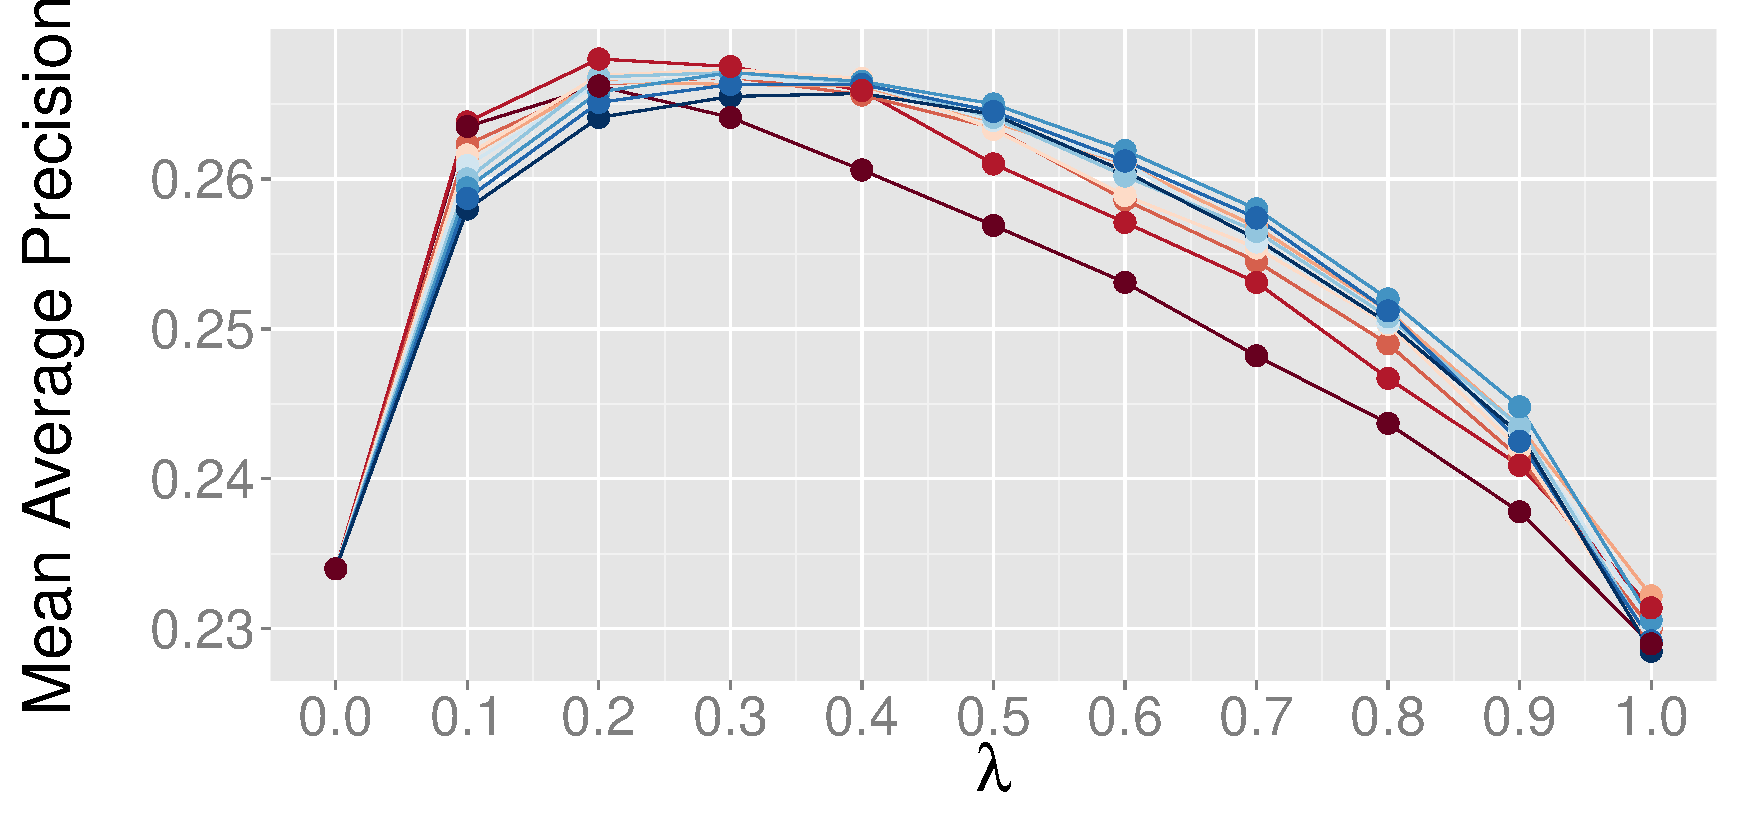
\includegraphics[width=\columnwidth]{figures/sweep-entities-AP.pdf}
\end{subfigure}%
\begin{subfigure}{.5\columnwidth}
\centering
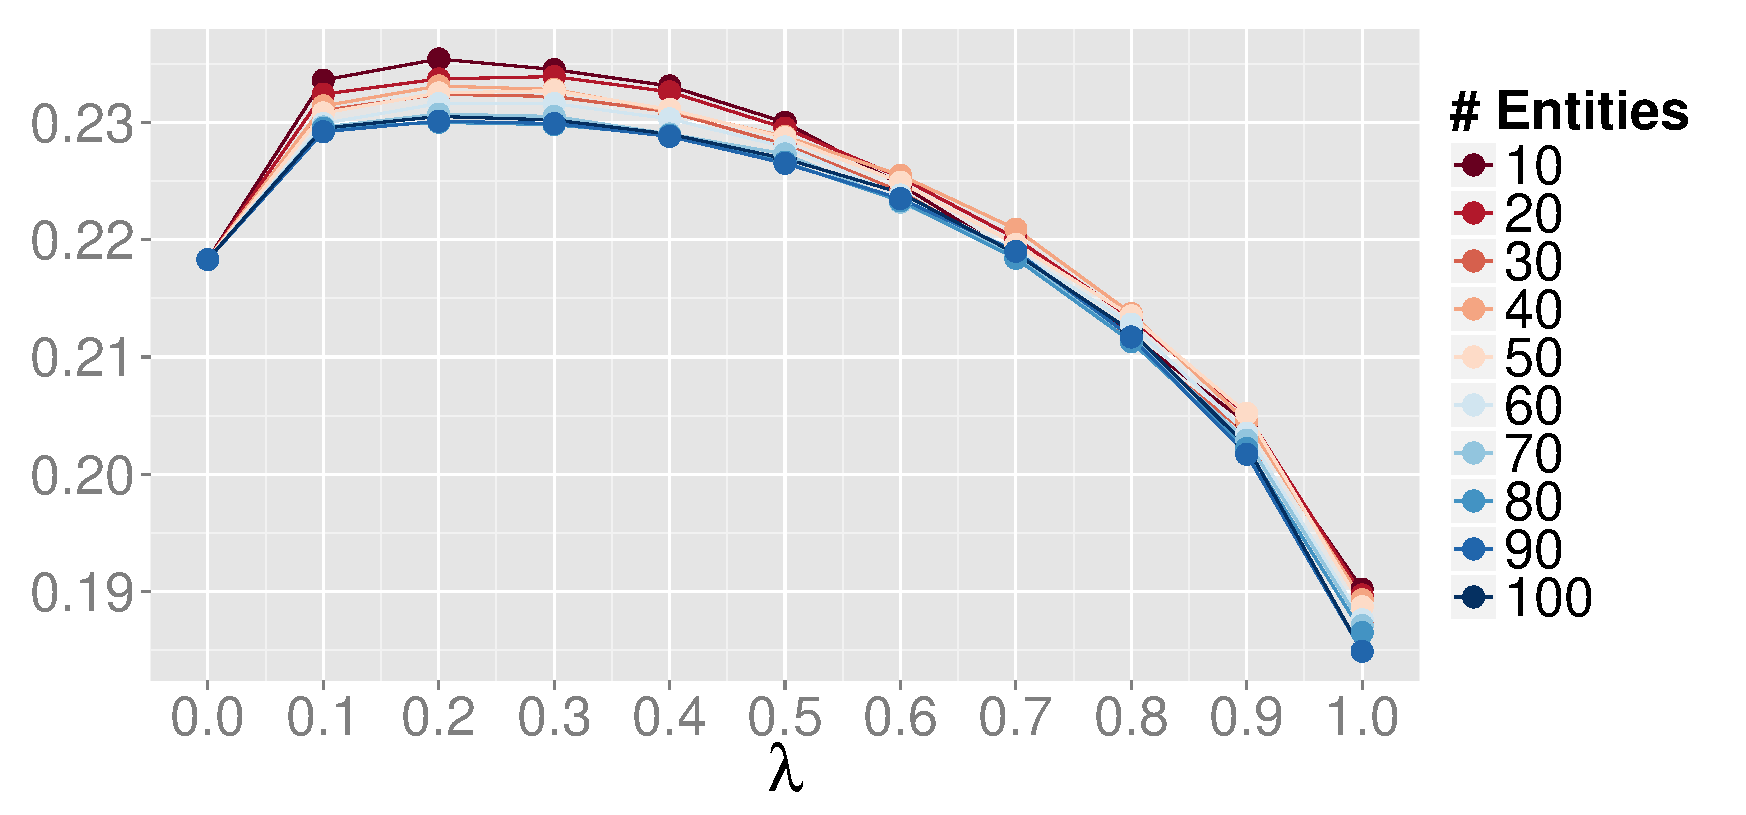
\includegraphics[width=\columnwidth]{figures/sweep-entities-robust.pdf}
\end{subfigure}
\caption{\textbf{Relating to old work, probably suggestive of this work, though:} Sweeps over values of $\lambda$ for AP (a) and robust (b) \textit{exp} runs. $\lambda=0.0$ is equivalent to the baseline run.}
\label{figure.sweeps-ql}
\end{figure*}

\section{Evaluation}\label{section.evaluation}

\subsection{Data}\label{section.evaluation.collections}

Although Eq. \ref{eq.ql-and-expansion-mult} allows for an arbitrary number of collections, for now we limit ourselves to two: the collection that the document appears in and Wikipedia. To this end, we make use of the September 1, 2015 dump of English Wikipedia. We build an Indri\footnote{http://www.lemurproject.org/indri/} index over the Wikipedia page text. The text of each page serves as the ``description text'' used in Eq. \ref{eq.expansion-sum}.

We test our approach using several TREC datasets:
\begin{itemize}
	\item The \textbf{AP} newswire collection from TREC disks 1 and 2 with topics 101-200.
	\item The \textbf{robust} 2004 topics, numbering 250, from TREC disks 4 and 5.
	\item The \textbf{wt10g} collection with the 100 topics from the 2000 and 2001 TREC Web tracks.
	\item Topics 851-900 with the \textbf{blogs06} dataset.
	\item The \textbf{clueweb09} category B dataset with likely spam documents removed, topics 1-200.
\end{itemize}

These datasets were chosen because they provide a good range of collection types, from relatively homogeneous and small with well-formed documents (AP) to heterogeneous and large with varied document quality (clueweb09).

%For comparison, we also report the results of our model using entity links produced by Apache Stanbol\footnote{http://stanbol.apache.org/}. We process the test collections with Stanbol's default ``enhancer,'' which supplies entity links and corresponding confidence scores. Stanbol's links to DBpedia\footnote{http://dbpedia.org} generally correspond to Wikipedia pages and may be converted easily. We select the link with the highest confidence for each mention in a given document and limit the set of links to $n$, the number of entities used in our bag-of-links approach. These links form the set of document links, and their confidence scores are normalized to provide an estimate of $P(E|D)$.

\subsection{Runs}\label{section.evaluation.runs}

%In some of the following runs, we make use of the RM3 variant of relevance modeling \cite{Lavrenko2001} which interpolates the original query $Q$ with the relevance model using a mixing parameter $\alpha$. RM3 provides a stronger baseline than standard query likelihood.

We produce three runs per collection:
\begin{itemize}
	\item \textit{baseline-ql}, a baseline query likelihood run
	\item \textit{baseline-rm3}, a baseline RM3 run
	\item \textit{exp-ql}, incorporating expansion documents using Eq. \ref{eq.ql-and-expansion}
%	\item \textit{stanbol-ql}, which uses Stanbol entity annotations in place of our document-level links.
\end{itemize}

We remove stop words in documents and entity descriptions for all runs. For the \textit{exp} runs, we retrieve the top 1000 documents per query using the default Indri query likelihood implementation. We then re-rank these documents by incorporating their knowledge base links as described in Section \ref{section.model}.

\subsection{Parameters}\label{section.evaluation.parameters}

\begin{table}[htb]
\centering
\begin{tabular}{|c|p{0.29\textwidth}|c|} \hline
{\bf Param} & {\bf Meaning} & {\bf Value} \\ \hline
$k$ & The maximum number of document terms to use in constructing $Q_D$. & 20 \\ \hline
$n$ & The maximum number of expansion documents in $\mathcal{E}_D$. & 10 \\ \hline
$\lambda_{\mathcal{E}_D}$ & One of several related mixing parameters controlling the weights of $P(q|D)$ and $P(q|\mathcal{E}_D)$ & 0.0-1.0 \\ \hline
$\mu$ & Used for Dirichlet smoothing of both $P(q|D)$ and $P(q|E)$. & 2500 \\ \hline
$fbDocs$ & The number of feedback documents to use for RM3 runs. & 20 \\ \hline
$fbTerms$ & The number of terms per document to use for RM3 runs. & 20 \\ \hline
$\alpha$ & Mixing parameter controlling the weights of the original query and relevance model for RM3 runs. & 0.0-1.0 \\ \hline
\end{tabular}
\caption{Parameter settings for the document expansion procedure and retrieval model}
\label{table.parameters}
\end{table}

The various parameters required for our approach, along with their meanings and the values used in our experiments, are shown in Table \ref{table.parameters}. 

%We sweep across values of $\lambda_{\mathcal{E}_D}$ and $n$ at intervals of 0.1 and 10 respectively to investigate the sensitivity of our model to these parameters. The results of these sweeps are shown in Figure \ref{figure.sweeps-ql} and discussed further in Section \ref{section.results}.

For this work, we set $k$ heuristically. In principle, this parameter need not be limited beyond the length of the document; however, this would increase computation time significantly, so we have opted to set it to the specified value.

\textbf{I have also set $n$ heuristically but intend to do a sweep over values of $n$ to ensure it is not a sensitive parameter. Prior work suggests it is not.}

%To set the two $\lambda_{\mathcal{E}_D}$ values, we use 5-fold cross validation. This entails splitting each set of topics into five random groups (folds) and using four of them in concert with relevance judgments to determine optimal parameter settings, which we test using the fifth. By using each of the five folds as the test fold once, we produce results that fully cover the topic set; we combine these results in order to perform batch evaluation. Additionally, since the quality of the results depends in part on the initial random fold creation, we run the cross-validation repeatedly 75 times and report the average metric across these repeated runs. This helps ensure that strong performance is not the result of a beneficial but random division of documents.

To set the two $\lambda_{\mathcal{E}_D}$ values, we use 5-fold cross validation. This entails splitting each set of topics into five random groups (folds) and using four of them in concert with relevance judgments to determine optimal parameter settings, which we test using the fifth. By using each of the five folds as the test fold once, we produce results that fully cover the topic set; we combine these results in order to perform batch evaluation. 

\section{Results}\label{section.results}

\begin{table}[htbp]
\centering
\begin{tabular}{|c|l|c|c|} \hline
{\bf Collection} & {\bf Run} & {\bf MAP} & {\bf nDCG@20} \\ \hline\hline
\rule{0pt}{2.5ex} \multirow{3}{*}{AP} & {\it baseline-ql} & 0.2337 & 0.4170 \\ \cline{2-4}
\rule{0pt}{2.5ex} & {\it baseline-rm} & 0.3298 ($\alpha=0.2$) & 0.4852 ($\alpha=0.3$) \\ \cline{2-4}
\rule{0pt}{2.5ex} & {\it baseline-rm-cv} & 0.3291 & 0.4858 \\ \cline{2-4}
\rule{0pt}{2.5ex} & {\it exp-ql} & ?? & ?? \\ \hline\hline
\rule{0pt}{2.5ex} \multirow{3}{*}{Robust} & {\it baseline-ql} & 0.2185 & 0.3825 \\ \cline{2-4}
\rule{0pt}{2.5ex} & {\it baseline-rm} & 0.2349 ($\alpha=0.2$) & 0.3893 ($\alpha=0.6$) \\ \cline{2-4}
\rule{0pt}{2.5ex} & {\it baseline-rm-cv} & 0.2663 & 0.3940 \\ \cline{2-4}
\rule{0pt}{2.5ex} & {\it exp-ql} & 0.2420$^{\Downarrow}$ & 0.4066$^{\uparrow}$ \\ \hline\hline
\rule{0pt}{2.5ex} \multirow{3}{*}{wt10g} & {\it baseline-ql} & 0.1687 & 0.2753 \\ \cline{2-4}
\rule{0pt}{2.5ex} & {\it baseline-rm} & 0.1735 ($\alpha=0.7,0.8$) & 0.2738 ($\alpha=1.0$)\\ \cline{2-4}
\rule{0pt}{2.5ex} & {\it baseline-rm-cv} & 0.1683 & 0.2633 \\ \cline{2-4}
\rule{0pt}{2.5ex} & {\it exp-ql} & 0.1827 & 0.3153$^{\uparrow\Uparrow}$ \\ \hline\hline
\rule{0pt}{2.5ex} \multirow{3}{*}{blogs06} & {\it baseline-ql} & 0.3064 & 0.2415 \\ \cline{2-4}
\rule{0pt}{2.5ex} & {\it baseline-rm} & 0.3103 ($\alpha=0.7$) & 0.2431 ($\alpha=1.0$)\\ \cline{2-4}
\rule{0pt}{2.5ex} & {\it baseline-rm-cv} & 0.3064 & 0.2330 \\ \cline{2-4}
\rule{0pt}{2.5ex} & {\it exp-ql} & 0.2988 & 0.2365 \\ \hline\hline
\rule{0pt}{2.5ex} \multirow{3}{*}{clueweb09} & {\it baseline-ql} & 0.1117 & 0.1944 \\ \cline{2-4}
\rule{0pt}{2.5ex} & {\it baseline-rm} & 0.1163 ($\alpha=0.2$) & 0.2034 ($\alpha=0.7$) \\ \cline{2-4}
\rule{0pt}{2.5ex} & {\it baseline-rm-cv} & ?? & ?? \\ \cline{2-4}
\rule{0pt}{2.5ex} & {\it exp-ql} & 0.1183$^{\uparrow}$ & 0.2100 \\ \hline
\end{tabular}
\caption{The top-scoring runs and baselines by MAP. $\uparrow$ indicates statistically significant improvements over the oracle RM3 baseline, \textit{baseline-rm}, while $\Uparrow$ and $\Downarrow$ indicate statistically significant improvement and decrease compared to the cross validated RM3 baseline, \textit{baseline-rm-cv}. Significance at $p < 0.05$.}
\label{table.performance}
\end{table}

Retrieval performance of the baselines and top-scoring runs are shown in Table \ref{table.performance}. Mean average precision (MAP) and normalized discounted cumulative gain at 20 (nDCG@20) scores marked with $\uparrow$ are greater than the optimal RM3 run with statistical significance at $p < 0.05$ using a paired one-tailed t-test. We also run a more realistic RM3 run using 10-fold cross validation to set the mixing parameter $\alpha$. Scores marked with $\Uparrow and \Downarrow$ signal statistically significant increases and decreases in performance relative to this cross validated RM3 run. Note that baselines correspond to $\sum_{j=1}^n \lambda_{{\mathcal{E}_D}_j} = 0.0$. 

\textbf{Relating to old work, probably suggestive of this work, though:} As Figure \ref{figure.sweeps-ql} shows, performance of \textit{kb} runs is not very sensitive to $n$, the number of linked entities: AP shows improvement over the baseline at $0.1 \leq \lambda \leq 0.9$ and robust at $0.1 \leq \lambda \leq 0.7$ for all values of $n$. Optimal performance for both collections occurs at relatively small numbers of entities as shown in Table \ref{table.performance}; this is a convenient result since it allows for more efficient document expansion.

\subsection{Is Expansion Worthwhile?}\label{section.results.expansion}

\begin{table}[htbp]
\centering
\begin{tabular}{|l|c|c|c|c|} \hline
& \multicolumn{2}{c}{Self} & \multicolumn{2}{|c|}{Wikipedia} \\ \hline
{\bf Collection} & {\bf $\lambda$} & {\bf MAP} & {\bf $\lambda$} & {\bf MAP} \\ \hline
AP & ? & ? & 0.2 & 0.2662 \\ \hline
Robust & ? & ? & 0.2 & 0.2354 \\ \hline
wt10g & ? & ? & ? & ? \\ \hline
blogs06 & ? & ? & ? & ? \\ \hline
clueweb09 & ? & ? & ? & ? \\ \hline
\end{tabular}
\caption{The top-scoring runs by MAP using only one collection of expansion documents. ``Self'' indicates expansion using the document's original collection while ``Wikipedia'' indicates expansion using Wikipedia.}
\label{table.performance.single}
\end{table}

\section{Conclusions}\label{section.conclusions}

The results indicate that our approach for expanding documents using Wikipedia and the document's original collection produces useful data for document retrieval purposes. Our simple document expansion model performs well compared to both a query likelihood and RM3 baseline.

In this paper, we have limited ourselves to using only two collections. However, future work may benefit from incorporating more collections to improve our language model estimates. Since our retrieval model performs \textit{document} expansion, we also plan to investigate its utility when paired with \textit{query} expansion techniques that employ knowledge base links.

\section{Acknowledgments}\label{section.acknowledgments}
This work was supported in part by the US National Science Foundation under Grant No. [blind]. Any opinions, findings, conclusions, or recommendations expressed are those of the authors and do not necessarily reflect the views of the National Science Foundation.


\bibliographystyle{abbrv}
\bibliography{library}  

\end{document}
